\begin{figure}[ht]
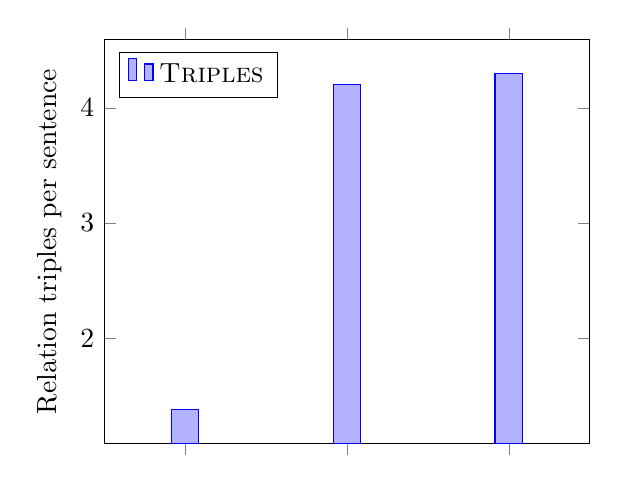
\begin{tikzpicture}
\begin{axis}[
    scale=0.9,
    ybar, 
    enlarge x limits={true, abs value=0.50},
    xtick=data,
    legend pos=north west,
    ylabel=Relation triples per sentence,
    xticklabels={
      \reverb, \openie, \openiecoref
    },
]
\addplot 
    coordinates {(1,1.38) (2,4.2) (3,4.3)};
            \addlegendentry{\textsc{Triples}}

\end{axis}
\end{tikzpicture}
  \caption{
    \label{fig:extrapolated}
    Compares the number of relation triples extracted per
    sentence. Both \openie systems achieve a similar result,
    while \reverb produces fewer triples per sentence.
  }
\end{figure}
